\chapter{Release 1 : Socle technique, Authentification et Gestion des Utilisateurs}
\label{chap:sprint_socle}

\section*{Introduction}
Ce troisi\`eme chapitre pr\'esente la r\'ealisation de la premi\`ere release du projet, correspondant aux it\'erations \textbf{S0 \`a S3}. Cette phase initiale a permis de mettre en place le socle architectural du projet, de d\'efinir les conventions de code et d'impl\'ementer le module critique de s\'ecurit\'e : l'authentification \`a deux niveaux (\textit{Access Token} \& \textit{Refresh Token}) et la gestion des comptes utilisateurs avec contr\^ole d'acc\`es bas\'e sur les r\^oles (\textit{Role-Based Access Control} -- RBAC) et le p\'erim\`etre r\'egional (\textit{Zone-Scoped Access}).

\section{Backlog de la Release 1}
Le tableau~\ref{tab:backlog-release1} d\'etaille le backlog de la release 1, prioris\'e selon la valeur m\'etier et technique.

\begin{table}[H]
\centering
\begin{tabular}{|p{8.5cm}|c|c|}
\hline
\textbf{\'El\'ement du Backlog} & \textbf{Priorit\'e} & \textbf{Sprint} \\
\hline
Initialisation de l'environnement, structure modulaire NestJS \& Flutter & Haute & S0 \\
\hline
Mod\'elisation des sch\'emas Mongoose et configuration de la base MongoDB & Haute & S1 \\
\hline
Impl\'ementation de l'authentification JWT (Access/Refresh Tokens) et hachage bcrypt & Haute & S2 \\
\hline
Mise en place des Guards RBAC et contr\^ole d'acc\`es par zone g\'eographique & Haute & S3 \\
\hline
D\'eveloppement des endpoints CRUD d'administration des utilisateurs & Haute & S3 \\
\hline
Int\'egration mobile : gestion de session Riverpod, stockage s\'ecuris\'e et GoRouter & Haute & S3 \\
\hline
\end{tabular}
\caption{Backlog d\'etaill\'e de la Release 1 (Sprints S0 \`a S3)}
\label{tab:backlog-release1}
\end{table}

\section{Raffinement des exigences et mod\'elisation UML}

\subsection{Module Authentification}

\subsubsection{Diagramme de cas d'utilisation}
La figure~\ref{fig:ch3-auth-usecase} illustre les fonctionnalit\'es li\'ees \`a l'acc\`es \`a la plateforme.

\begin{figure}[H]
 \centering
 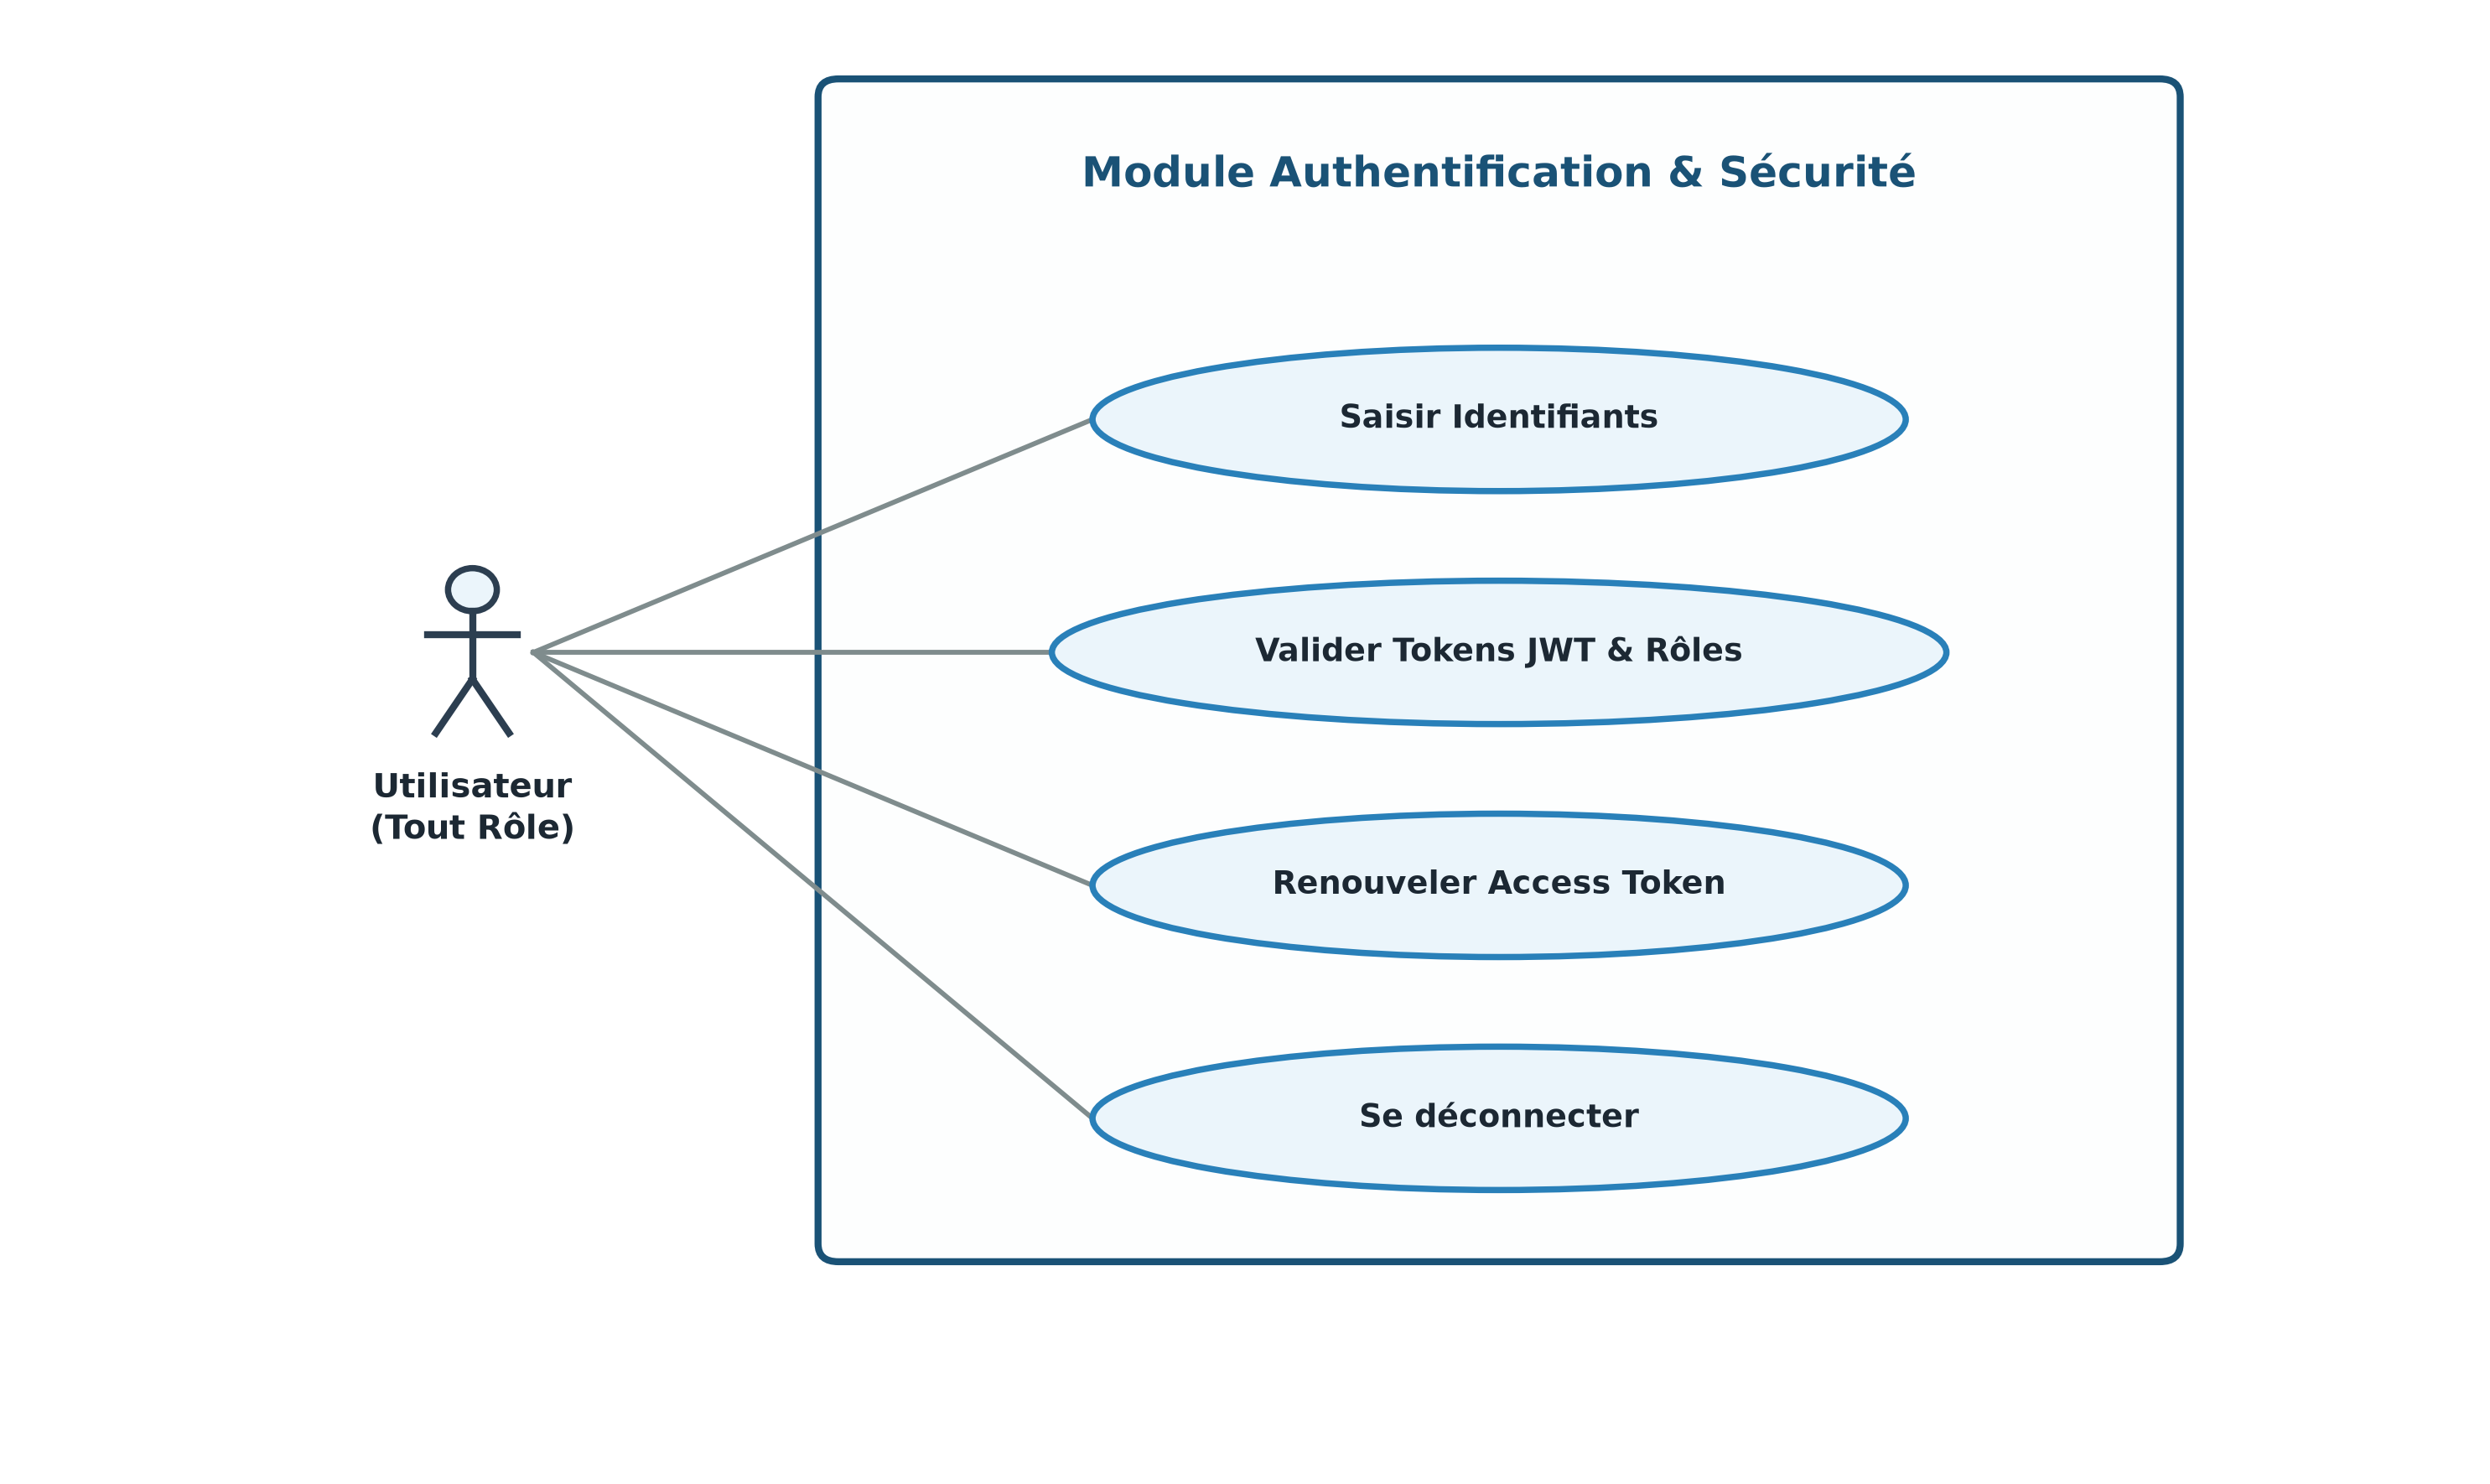
\includegraphics[width=11cm]{Images/ch3/auth_usecase.png}
 \caption{Diagramme de cas d'utilisation -- Module Authentification}
 \label{fig:ch3-auth-usecase}
\end{figure}

Le tableau~\ref{tab:ch3-auth-refinement} pr\'esente la sp\'ecification textuelle de l'authentification.

\begin{table}[H]
\centering
\begin{tabular}{|p{3.5cm}|p{10.5cm}|}
\hline
\textbf{Cas d'utilisation} & S'authentifier sur la plateforme \\
\hline
\textbf{Acteurs} & Administrateur, Responsable de zone, Technicien \\
\hline
\textbf{Pr\'econditions} & L'utilisateur dispose d'un compte actif cr\'e\'e par l'administrateur. \\
\hline
\textbf{Postconditions} & L'utilisateur re\c{c}oit un couple de jetons (\textit{AccessToken} \& \textit{RefreshToken}) et est redirig\'e vers l'\'ecran d'accueil autoris\'e selon son r\^ole. \\
\hline
\textbf{Sc\'enario nominal} & 
1. L'utilisateur saisit son email et son mot de passe sur l'application mobile. \newline
2. L'application transmet la requ\^ete au endpoint \texttt{/auth/login}. \newline
3. Le serveur NestJS v\'erifie les identifiants et compare le hachage bcrypt. \newline
4. Le serveur g\'en\`ere les tokens sign\'es et retourne le profil utilisateur. \newline
5. L'application stocke les jetons dans le coffre s\'ecuris\'e (\textit{flutter\_secure\_storage}) et initialise l'\'etat Riverpod. \\
\hline
\textbf{Sc\'enarios alternatifs} & Compte inactif ou mot de passe incorrect : le serveur renvoie un code HTTP 401 avec un message explicatif. \\
\hline
\end{tabular}
\caption{Description textuelle du cas d'utilisation « S'authentifier »}
\label{tab:ch3-auth-refinement}
\end{table}

\subsubsection{Diagramme de s\'equence de l'authentification}
La figure~\ref{fig:ch3-auth-seq} d\'etaille le cycle complet d'authentification et de s\'ecurisation des \'echanges entre l'application mobile Flutter, le serveur NestJS et la base MongoDB.

\begin{figure}[H]
 \centering
 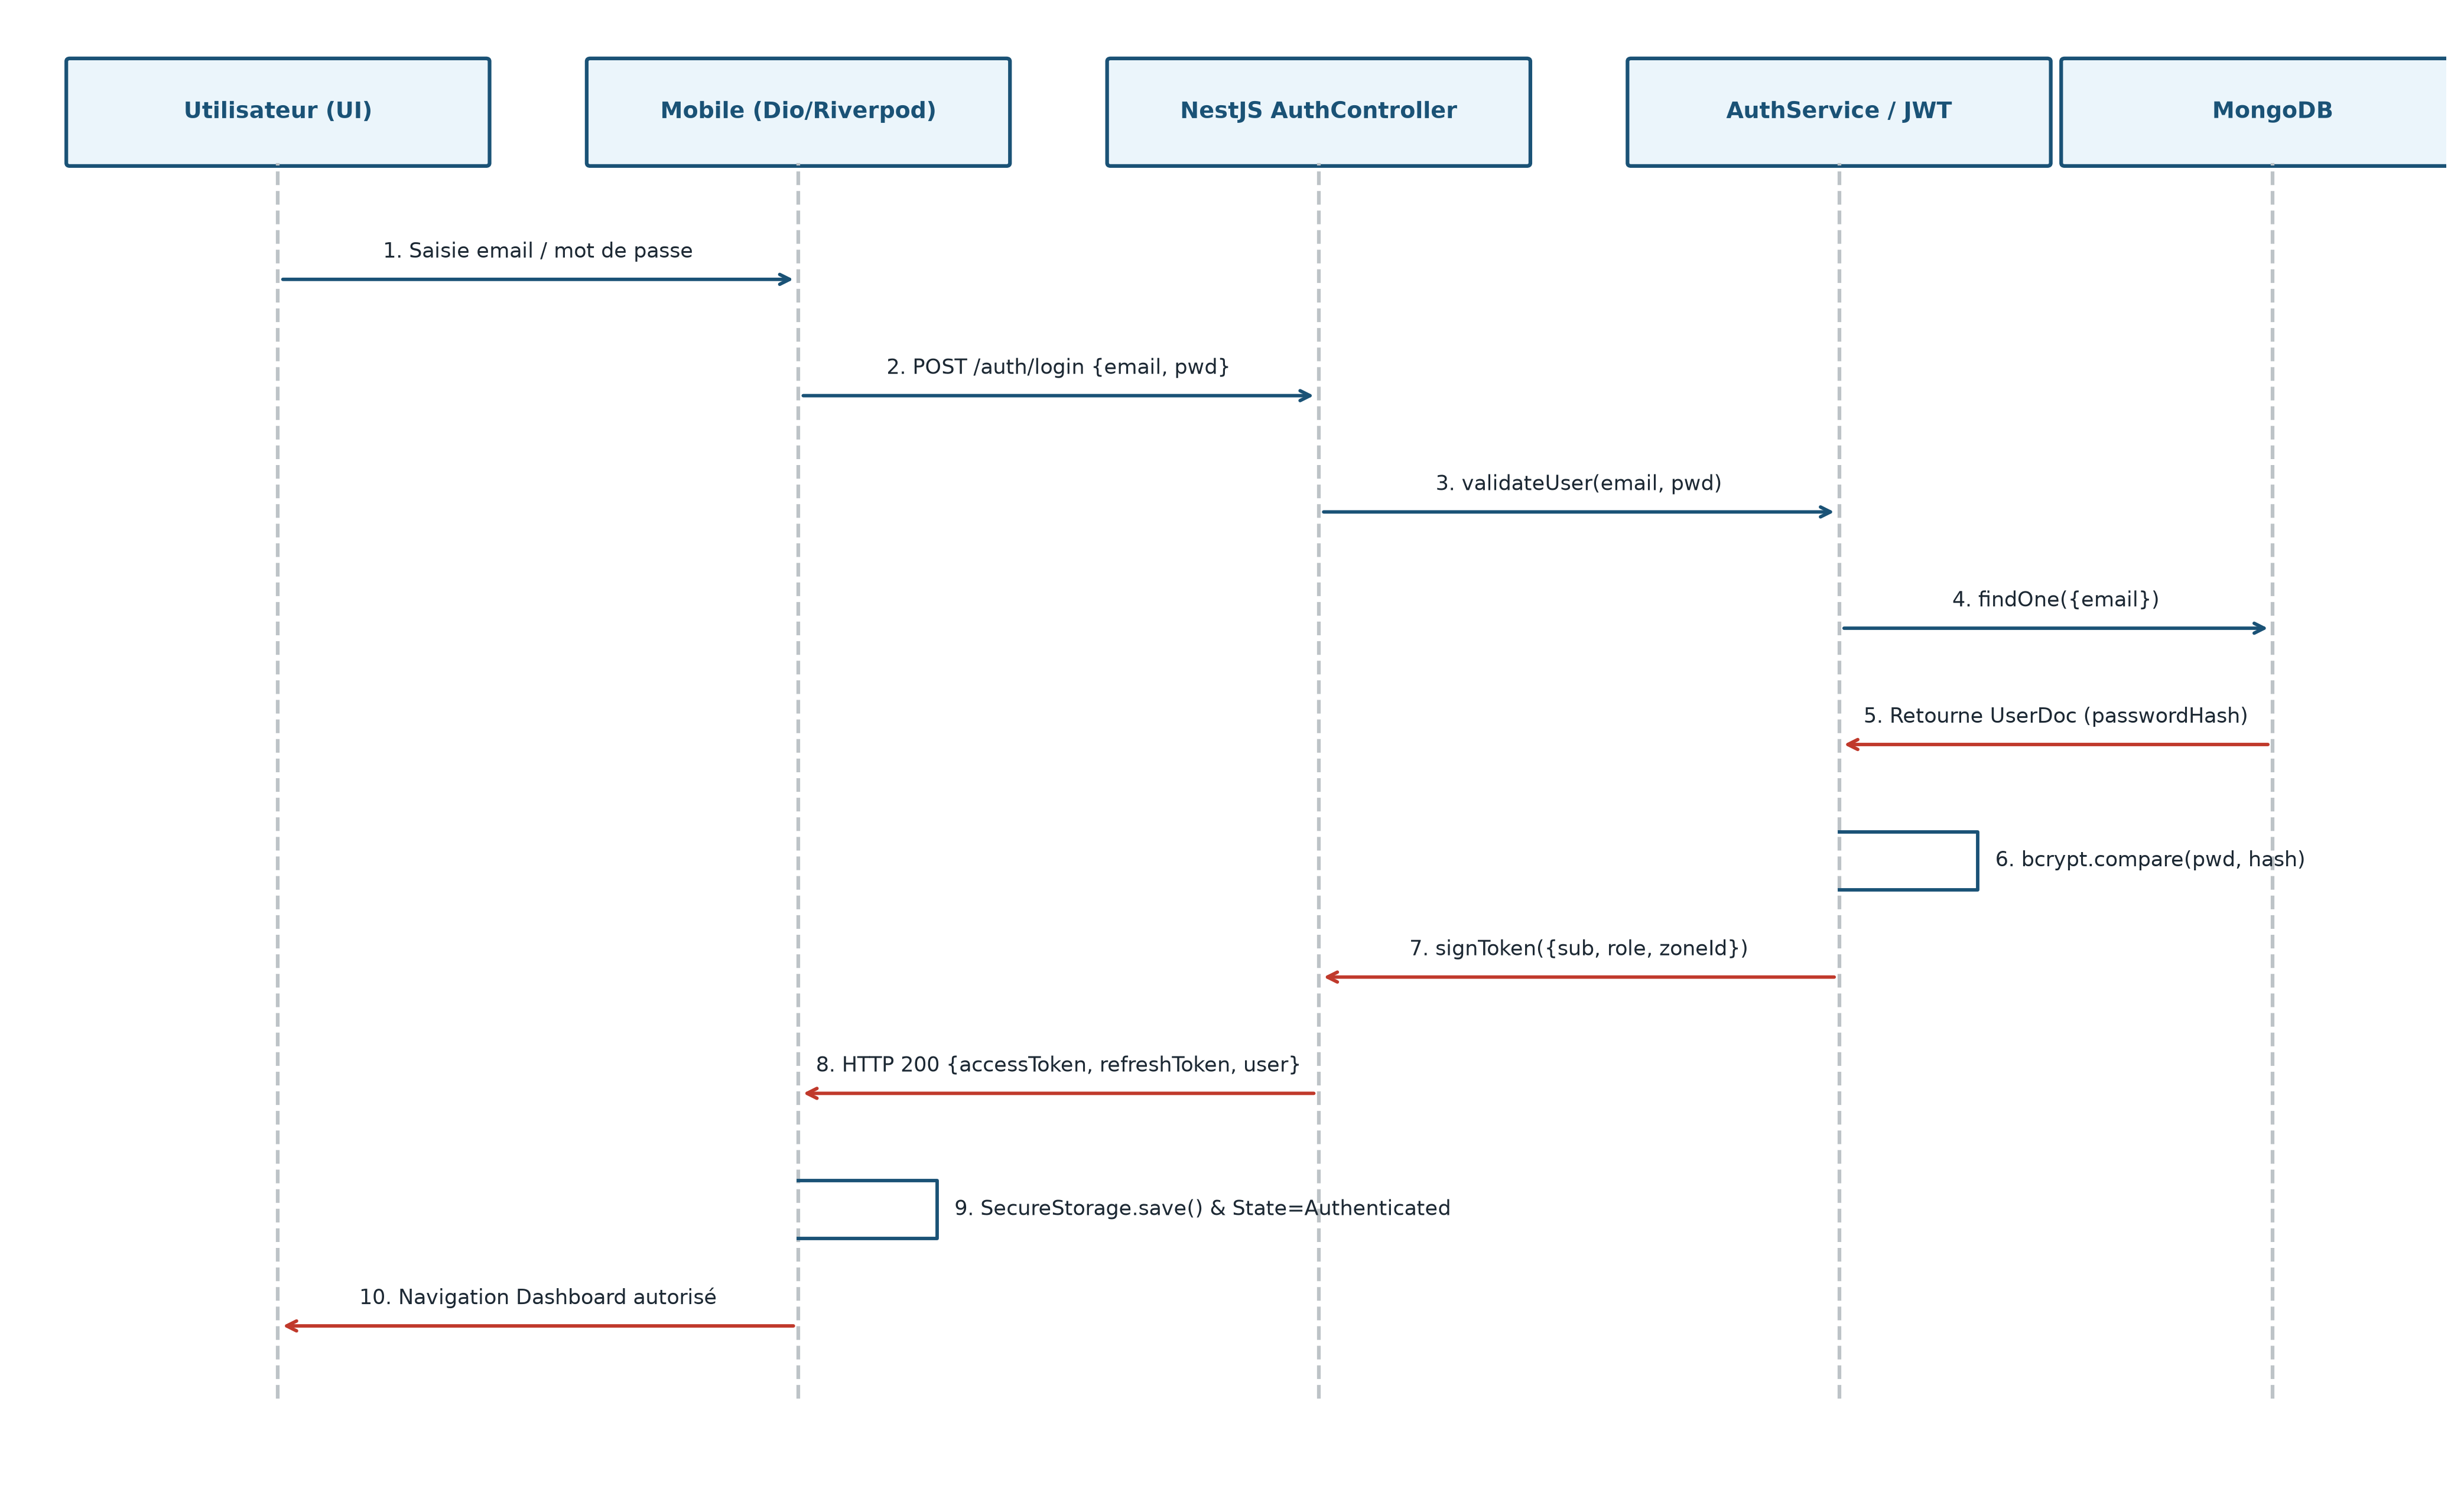
\includegraphics[width=15cm]{Images/ch3/auth_sequence.png}
 \caption{Diagramme de s\'equence -- Processus d'authentification s\'ecuris\'ee}
 \label{fig:ch3-auth-seq}
\end{figure}

\subsection{Module Gestion des Utilisateurs}

\subsubsection{Diagramme de cas d'utilisation global}
L'administration des utilisateurs et l'affectation des privil\`eges sont repr\'esent\'ees dans la figure~\ref{fig:ch3-users-global}.

\begin{figure}[H]
 \centering
 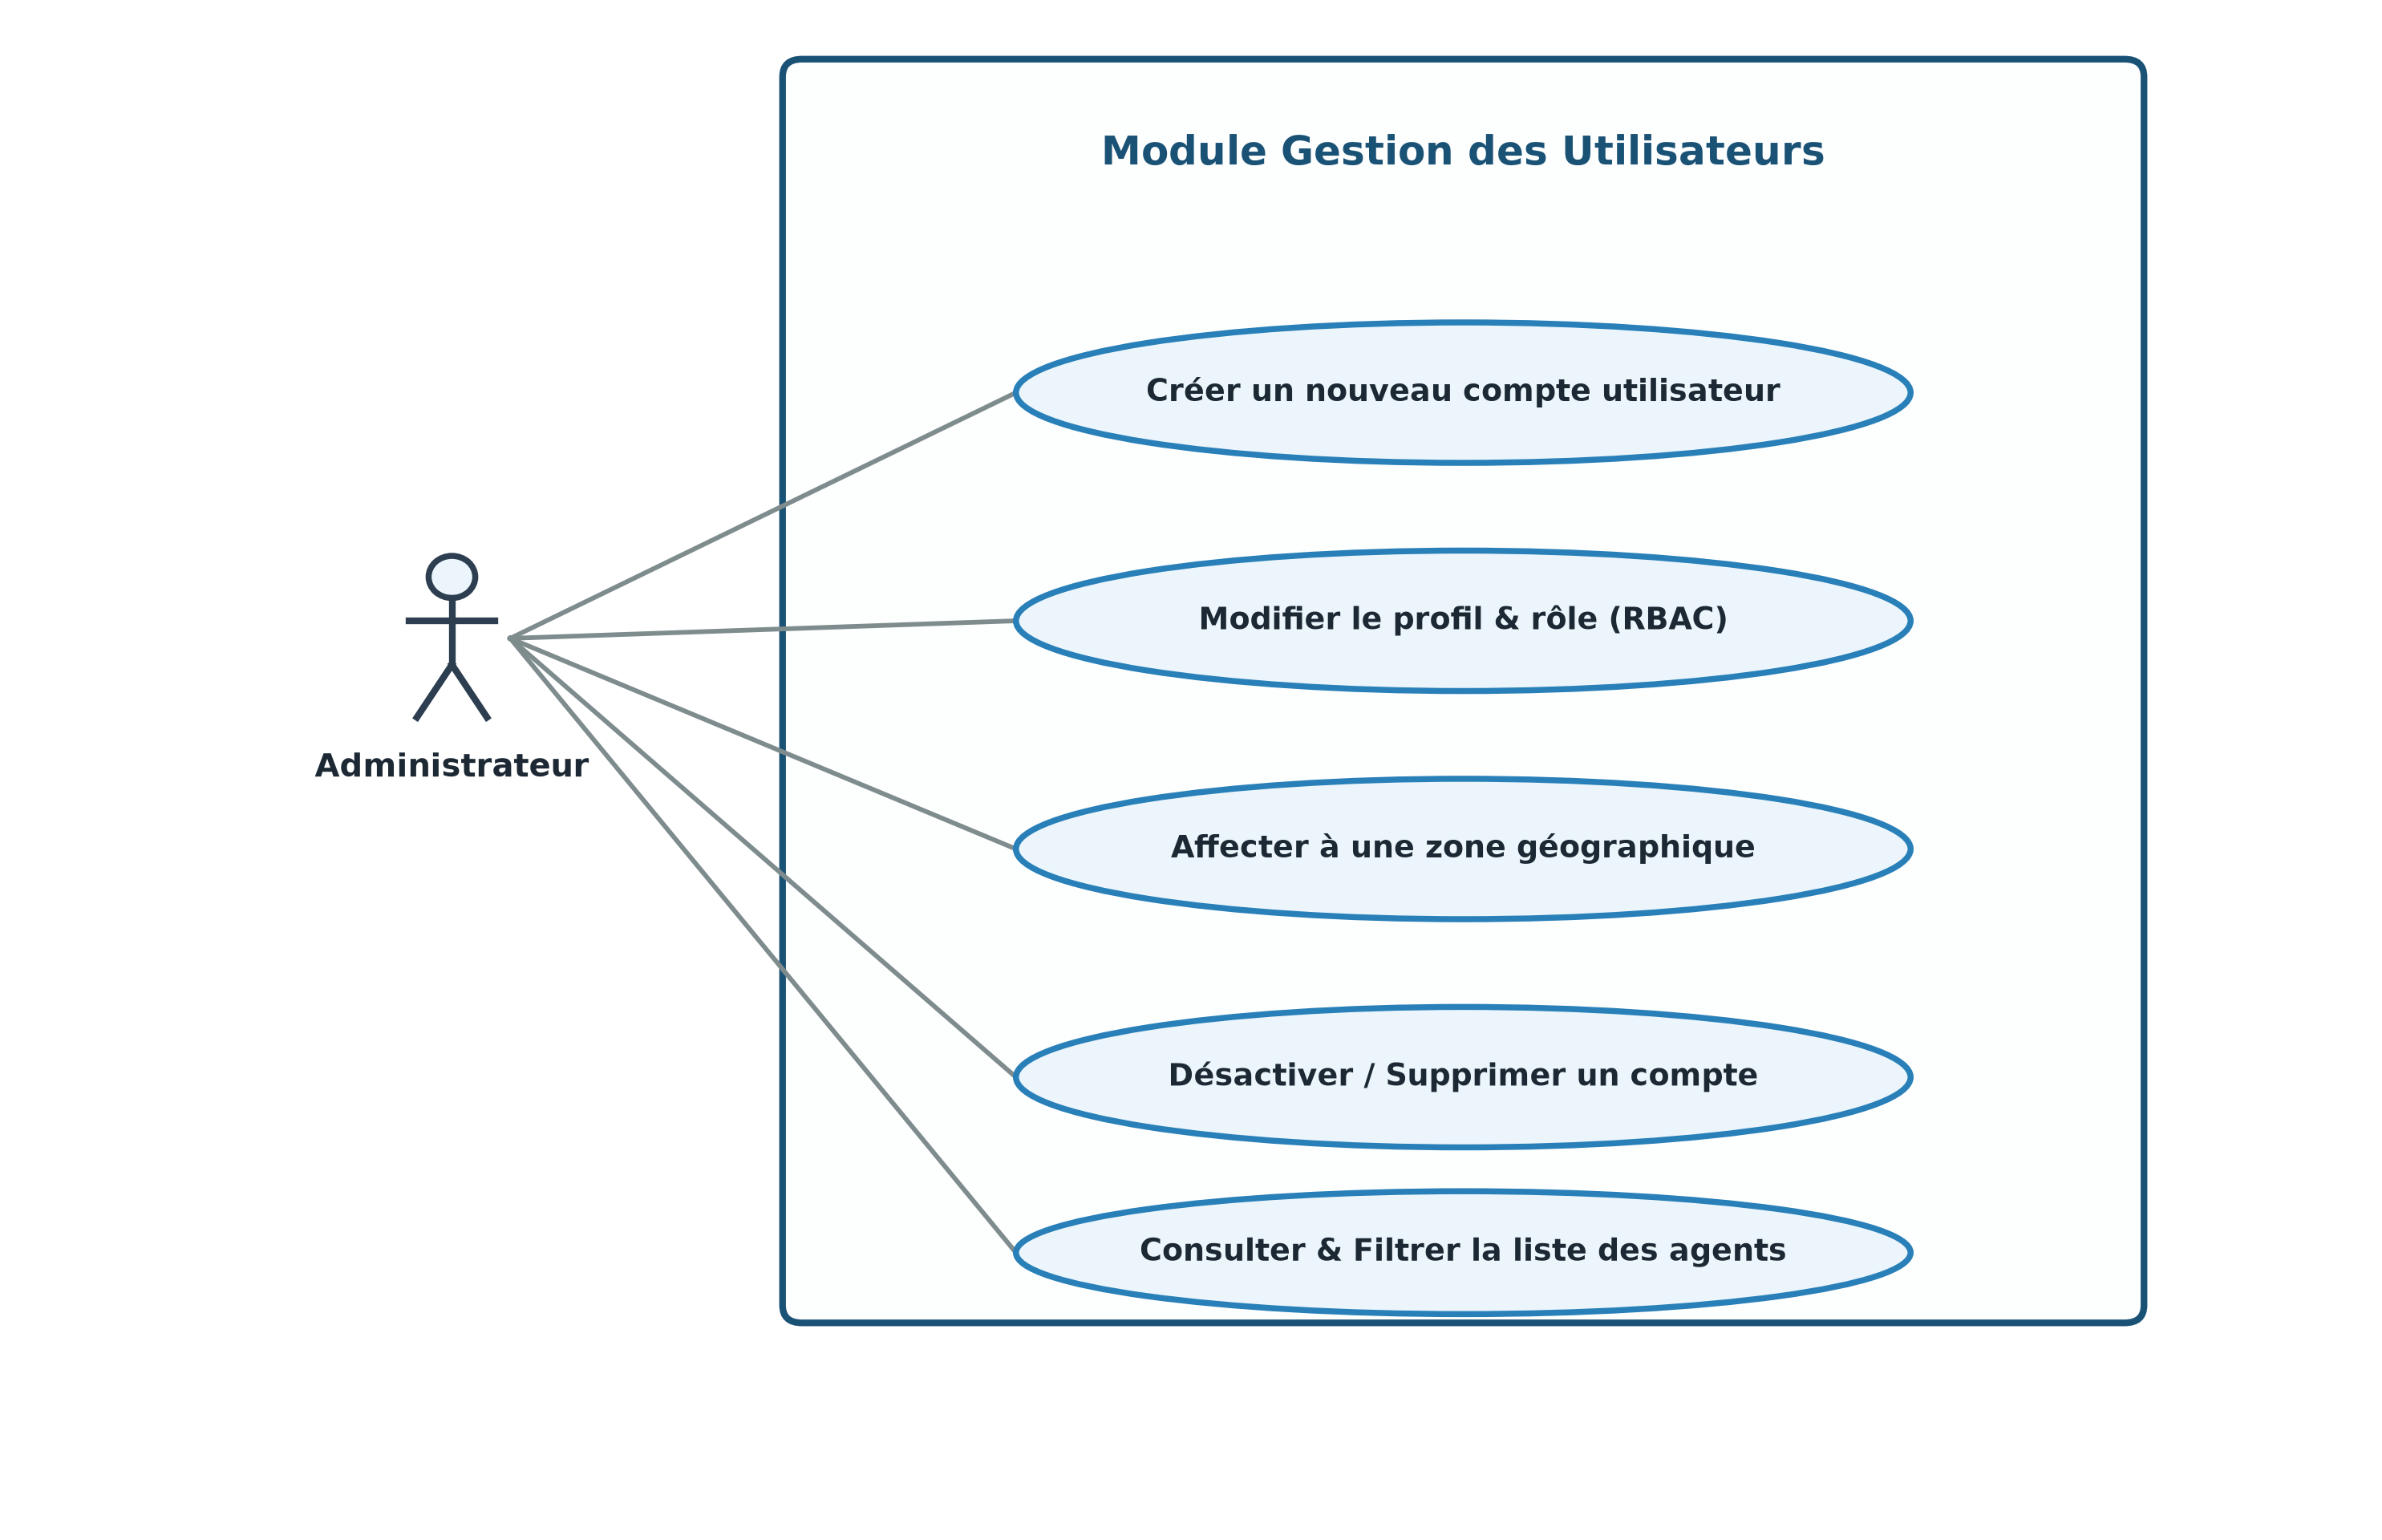
\includegraphics[width=12cm]{Images/ch3/users_global_usecase.png}
 \caption{Diagramme de cas d'utilisation -- Gestion des utilisateurs}
 \label{fig:ch3-users-global}
\end{figure}

\subsubsection{Diagramme de classes du domaine Utilisateur \& S\'ecurit\'e}
La figure~\ref{fig:ch3-auth-class} pr\'esente la structure des classes et des entit\'es de donn\'ees li\'ees \`a l'authentification, aux profils et aux r\^oles.

\begin{figure}[H]
 \centering
 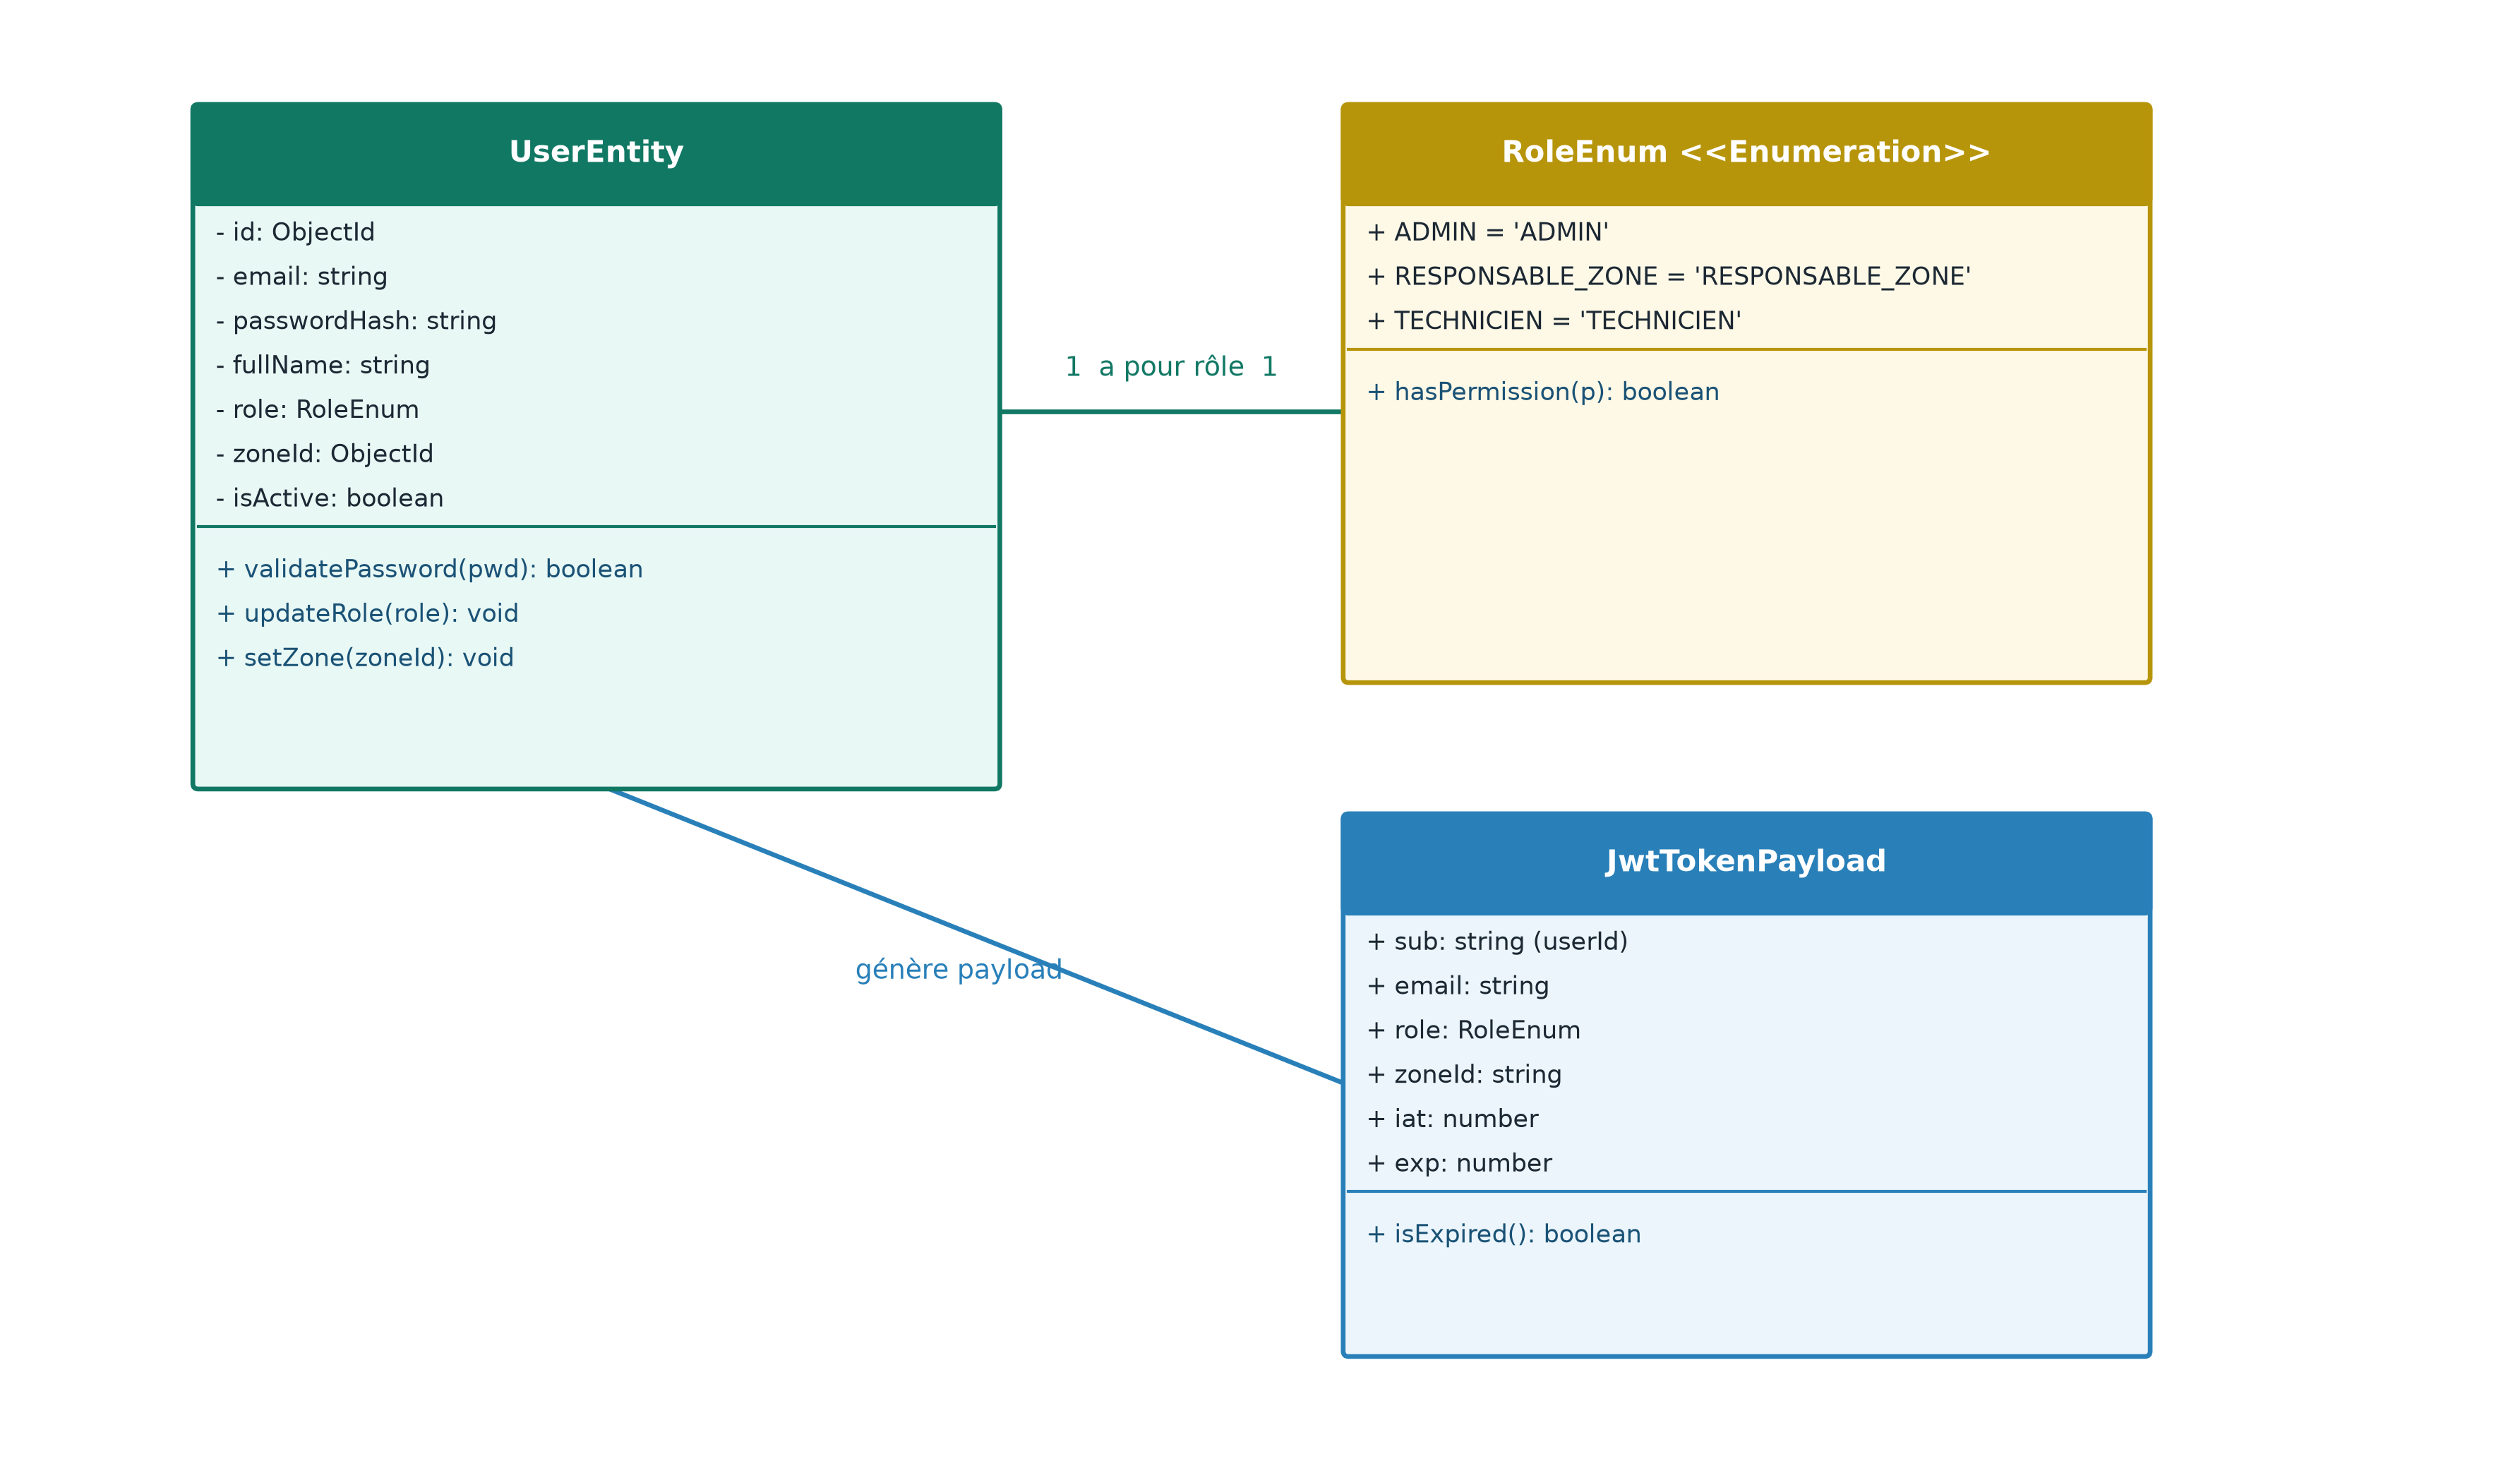
\includegraphics[width=13cm]{Images/ch3/auth_class.png}
 \caption{Diagramme de classes du domaine Utilisateur et S\'ecurit\'e}
 \label{fig:ch3-auth-class}
\end{figure}

\section{R\'ealisation technique et impl\'ementation}

\subsection{Impl\'ementation de la s\'ecurit\'e c\^ot\'e Back-End (NestJS)}
La s\'ecurisation du back-end s'appuie sur une combinaison de composants NestJS sp\'ecialis\'es :
\begin{itemize}
    \item \textbf{JwtAuthGuard :} Intercepte chaque requ\^ete entrante, extrait le jeton porteur (\textit{Bearer Token}) de l'en-t\^ete \texttt{Authorization}, et valide la signature cryptographique \`a l'aide de la cl\'e secr\`ete.
    \item \textbf{RolesGuard \& Decorator \texttt{@Roles()} :} V\'erifie que le r\^ole extrait du payload JWT correspond aux autorisations requises pour l'endpoint cible.
    \item \textbf{Hachage s\'ecuris\'e avec bcrypt :} Les mots de passe ne sont jamais stock\'es en clair ; un salage (\textit{salt rounds = 10}) est appliqu\'e avant persistance dans MongoDB.
    \item \textbf{Validation DTO :} Utilisation des d\'ecorateurs \texttt{class-validator} (\texttt{@IsEmail()}, \texttt{@IsNotEmpty()}) avec un \texttt{ValidationPipe} configur\'e en mode \texttt{whitelist: true} pour \'eliminer toute propri\'et\'e non d\'eclar\'ee (protection contre les injections de param\`etres).
\end{itemize}

\subsection{Impl\'ementation de la gestion de session c\^ot\'e Mobile (Flutter)}
L'application Flutter int\`egre une gestion d'\'etat r\'eactive robuste pour l'authentification :
\begin{itemize}
    \item \textbf{AuthNotifier (Riverpod) :} Notifie automatiquement toute l'arborescence des widgets des changements d'\'etat (\textit{authenticated}, \textit{unauthenticated}, \textit{loading}).
    \item \textbf{GoRouter Redirection :} Emp\^eche l'acc\`es aux \'ecrans internes tant que le jeton n'est pas valid\'e et oriente automatiquement l'utilisateur vers son tableau de bord d\'edi\'e selon son r\^ole.
    \item \textbf{Intercepteur Dio :} Capture les erreurs HTTP 401 (\textit{Token Expired}) et d\'eclenche de mani\`ere transparente le renouvellement via le \textit{Refresh Token} sans d\'econnecter l'utilisateur.
\end{itemize}

\subsection{Interfaces utilisateur r\'ealis\'ees}

\subsubsection{Interface de connexion}
La figure~\ref{fig:ch3-ui-login} pr\'esente l'\'ecran d'authentification mobile avec contr\^ole de saisie en temps r\'eel.

\begin{figure}[H]
 \centering
 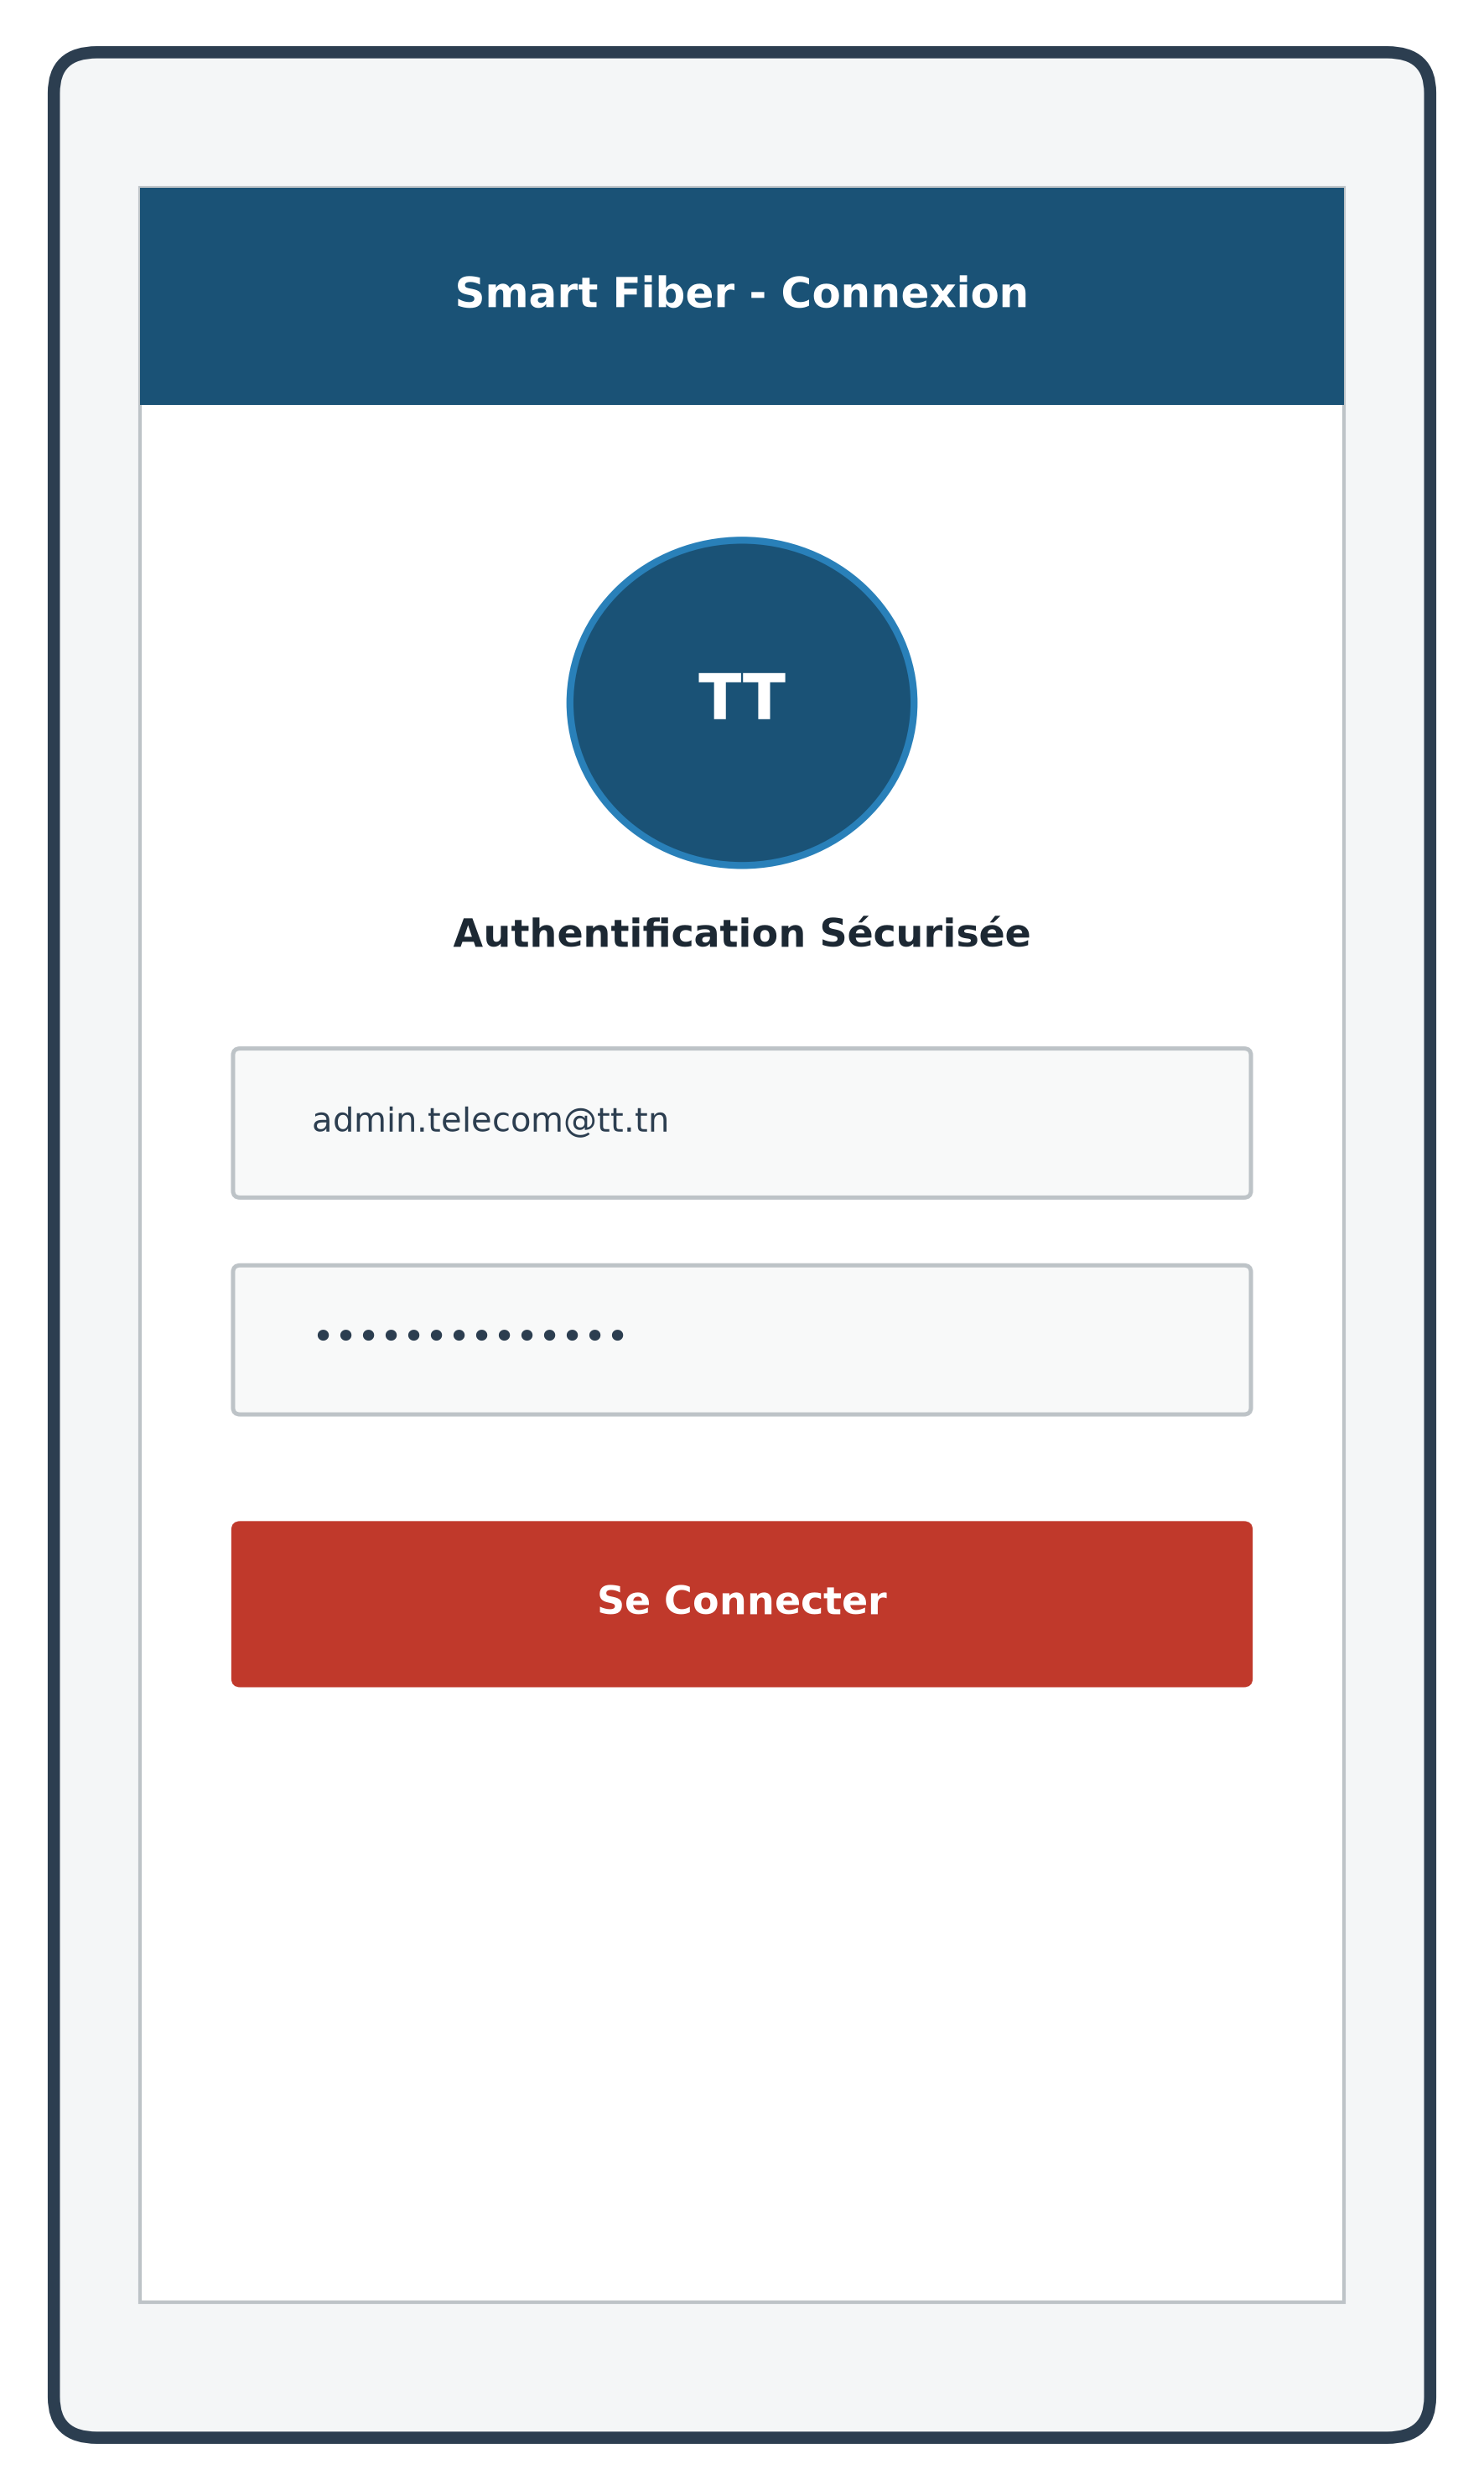
\includegraphics[width=10cm]{Images/ch3/ui_login.png}
 \caption{Interface mobile d'authentification}
 \label{fig:ch3-ui-login}
\end{figure}

\subsubsection{Interface de gestion des utilisateurs}
La figure~\ref{fig:ch3-ui-admin-users} illustre la liste des comptes utilisateurs avec filtres par r\^ole et zone, et la figure~\ref{fig:ch3-ui-create-user} montre le formulaire de cr\'eation avec s\'election du r\^ole et de la zone de rattachement.

\begin{figure}[H]
 \centering
 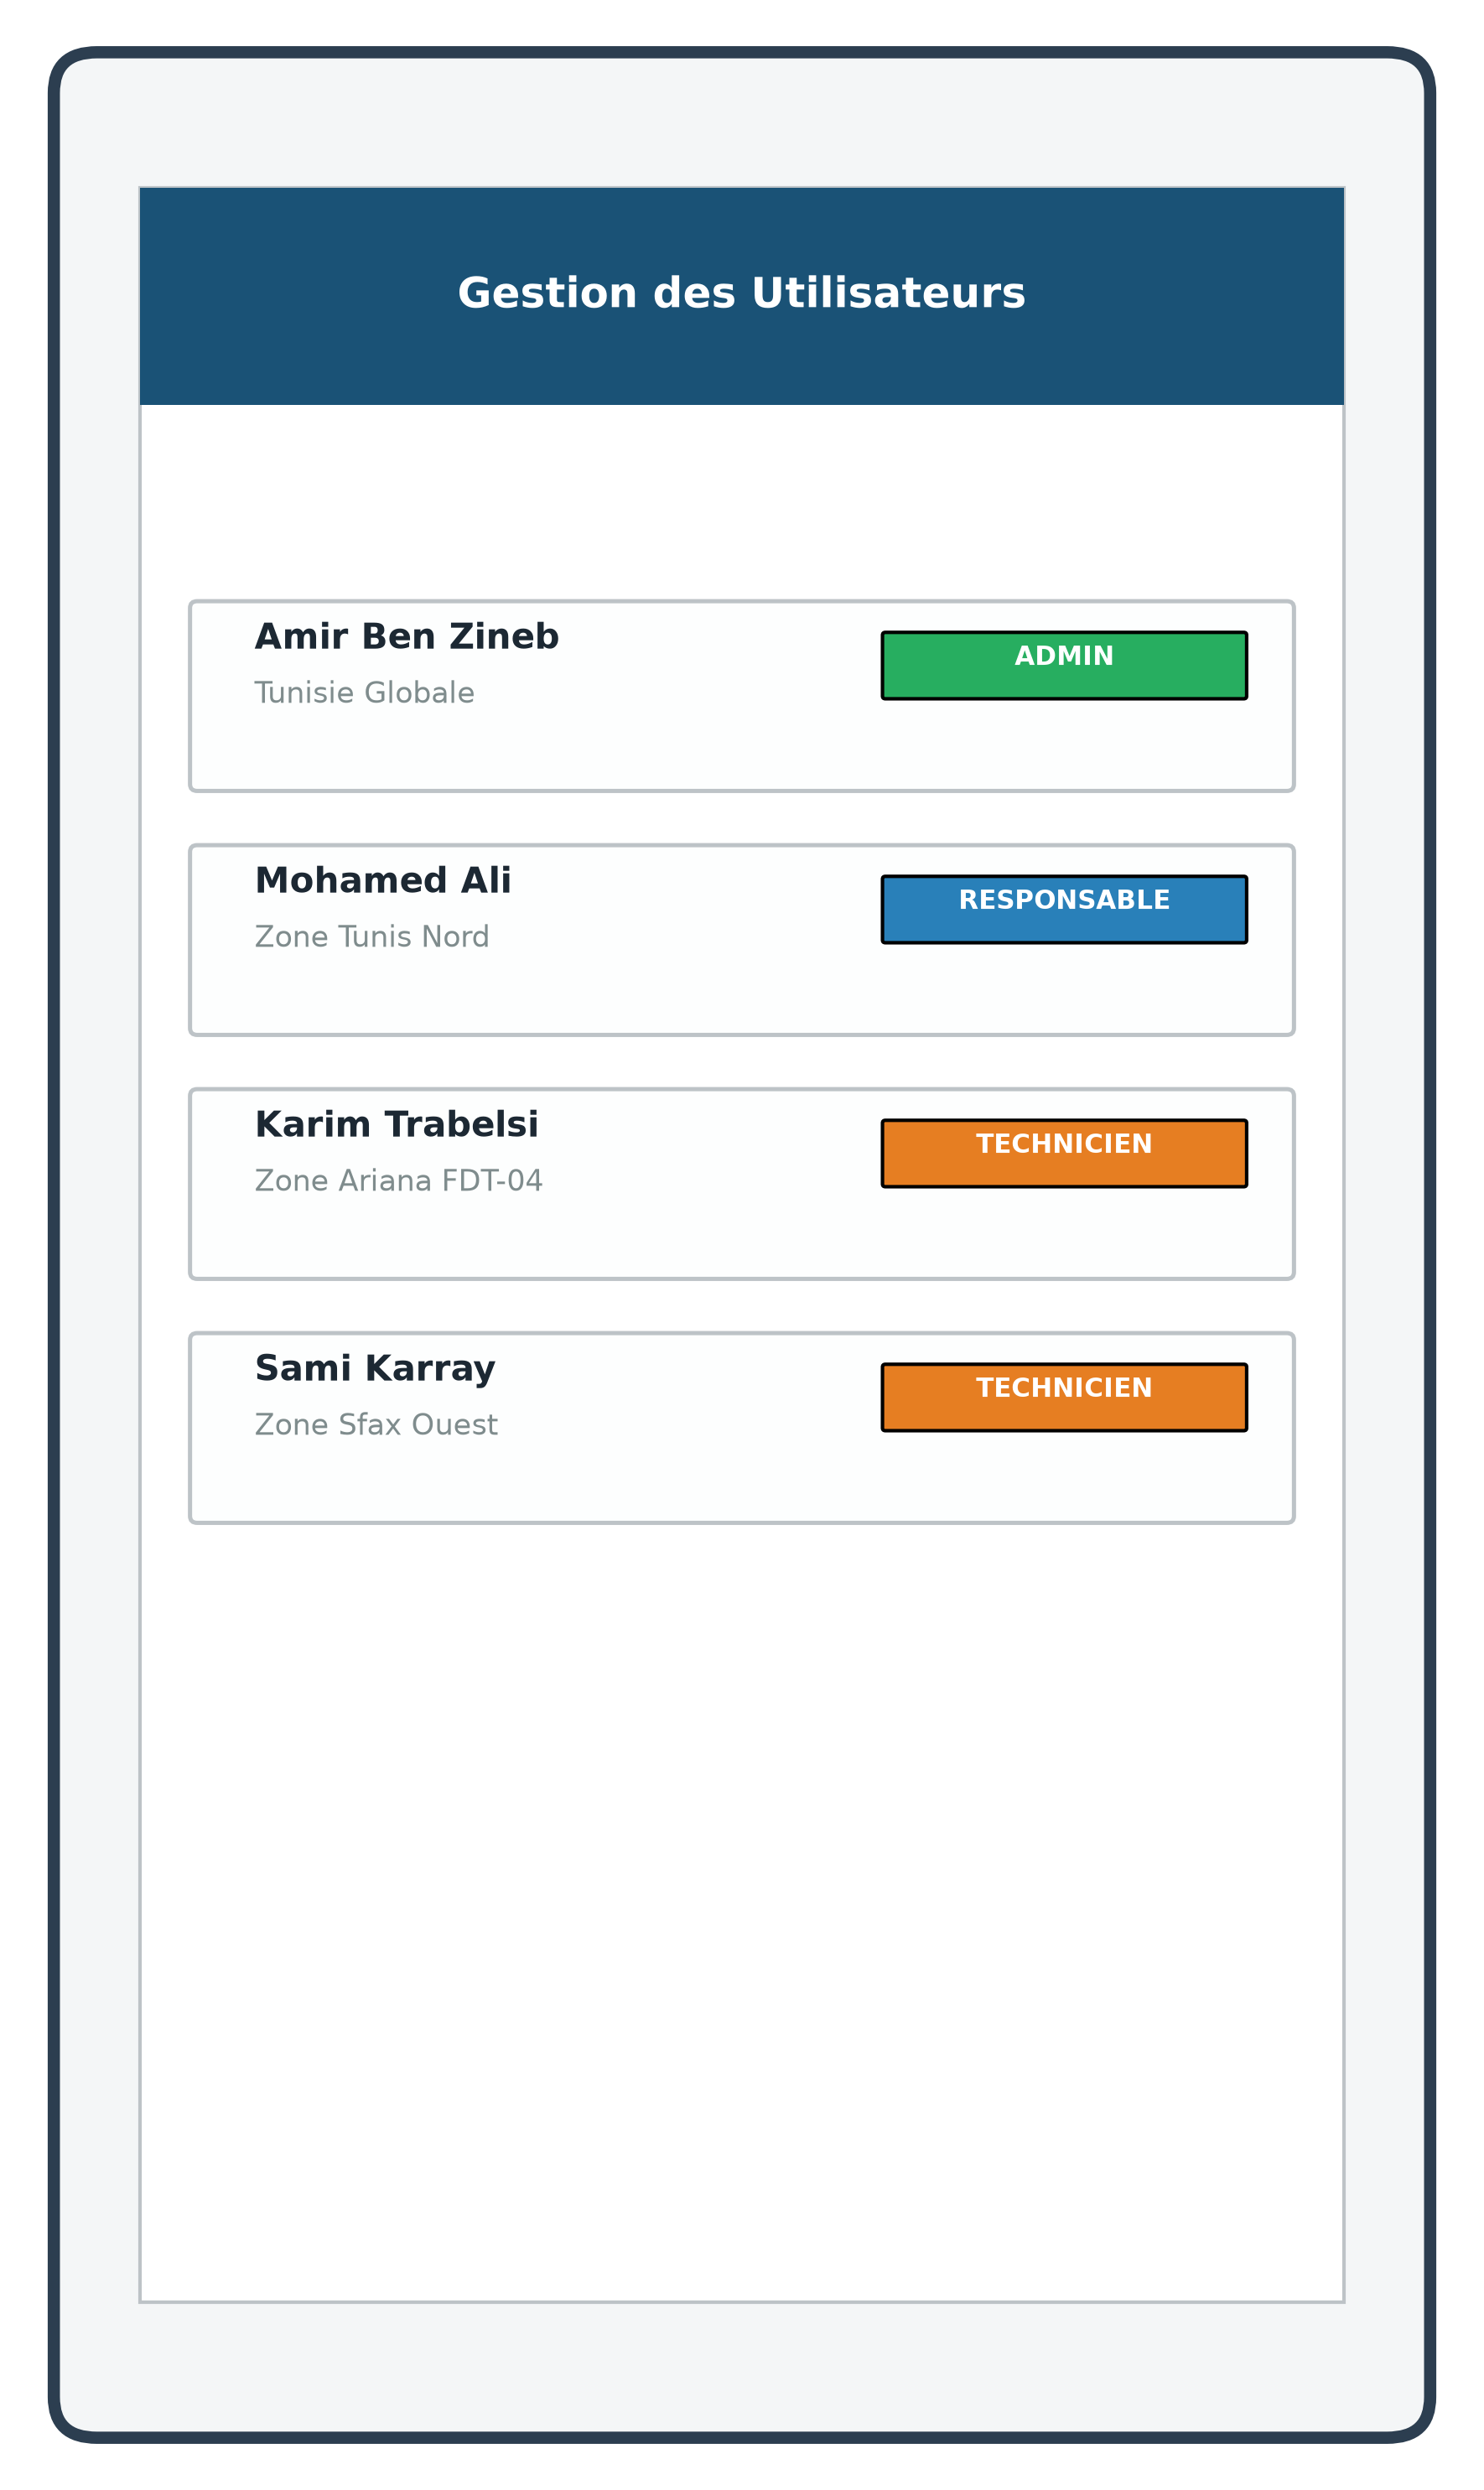
\includegraphics[width=13cm]{Images/ch3/ui_admin_users.png}
 \caption{Interface d'administration et consultation des utilisateurs}
 \label{fig:ch3-ui-admin-users}
\end{figure}

\begin{figure}[H]
 \centering
 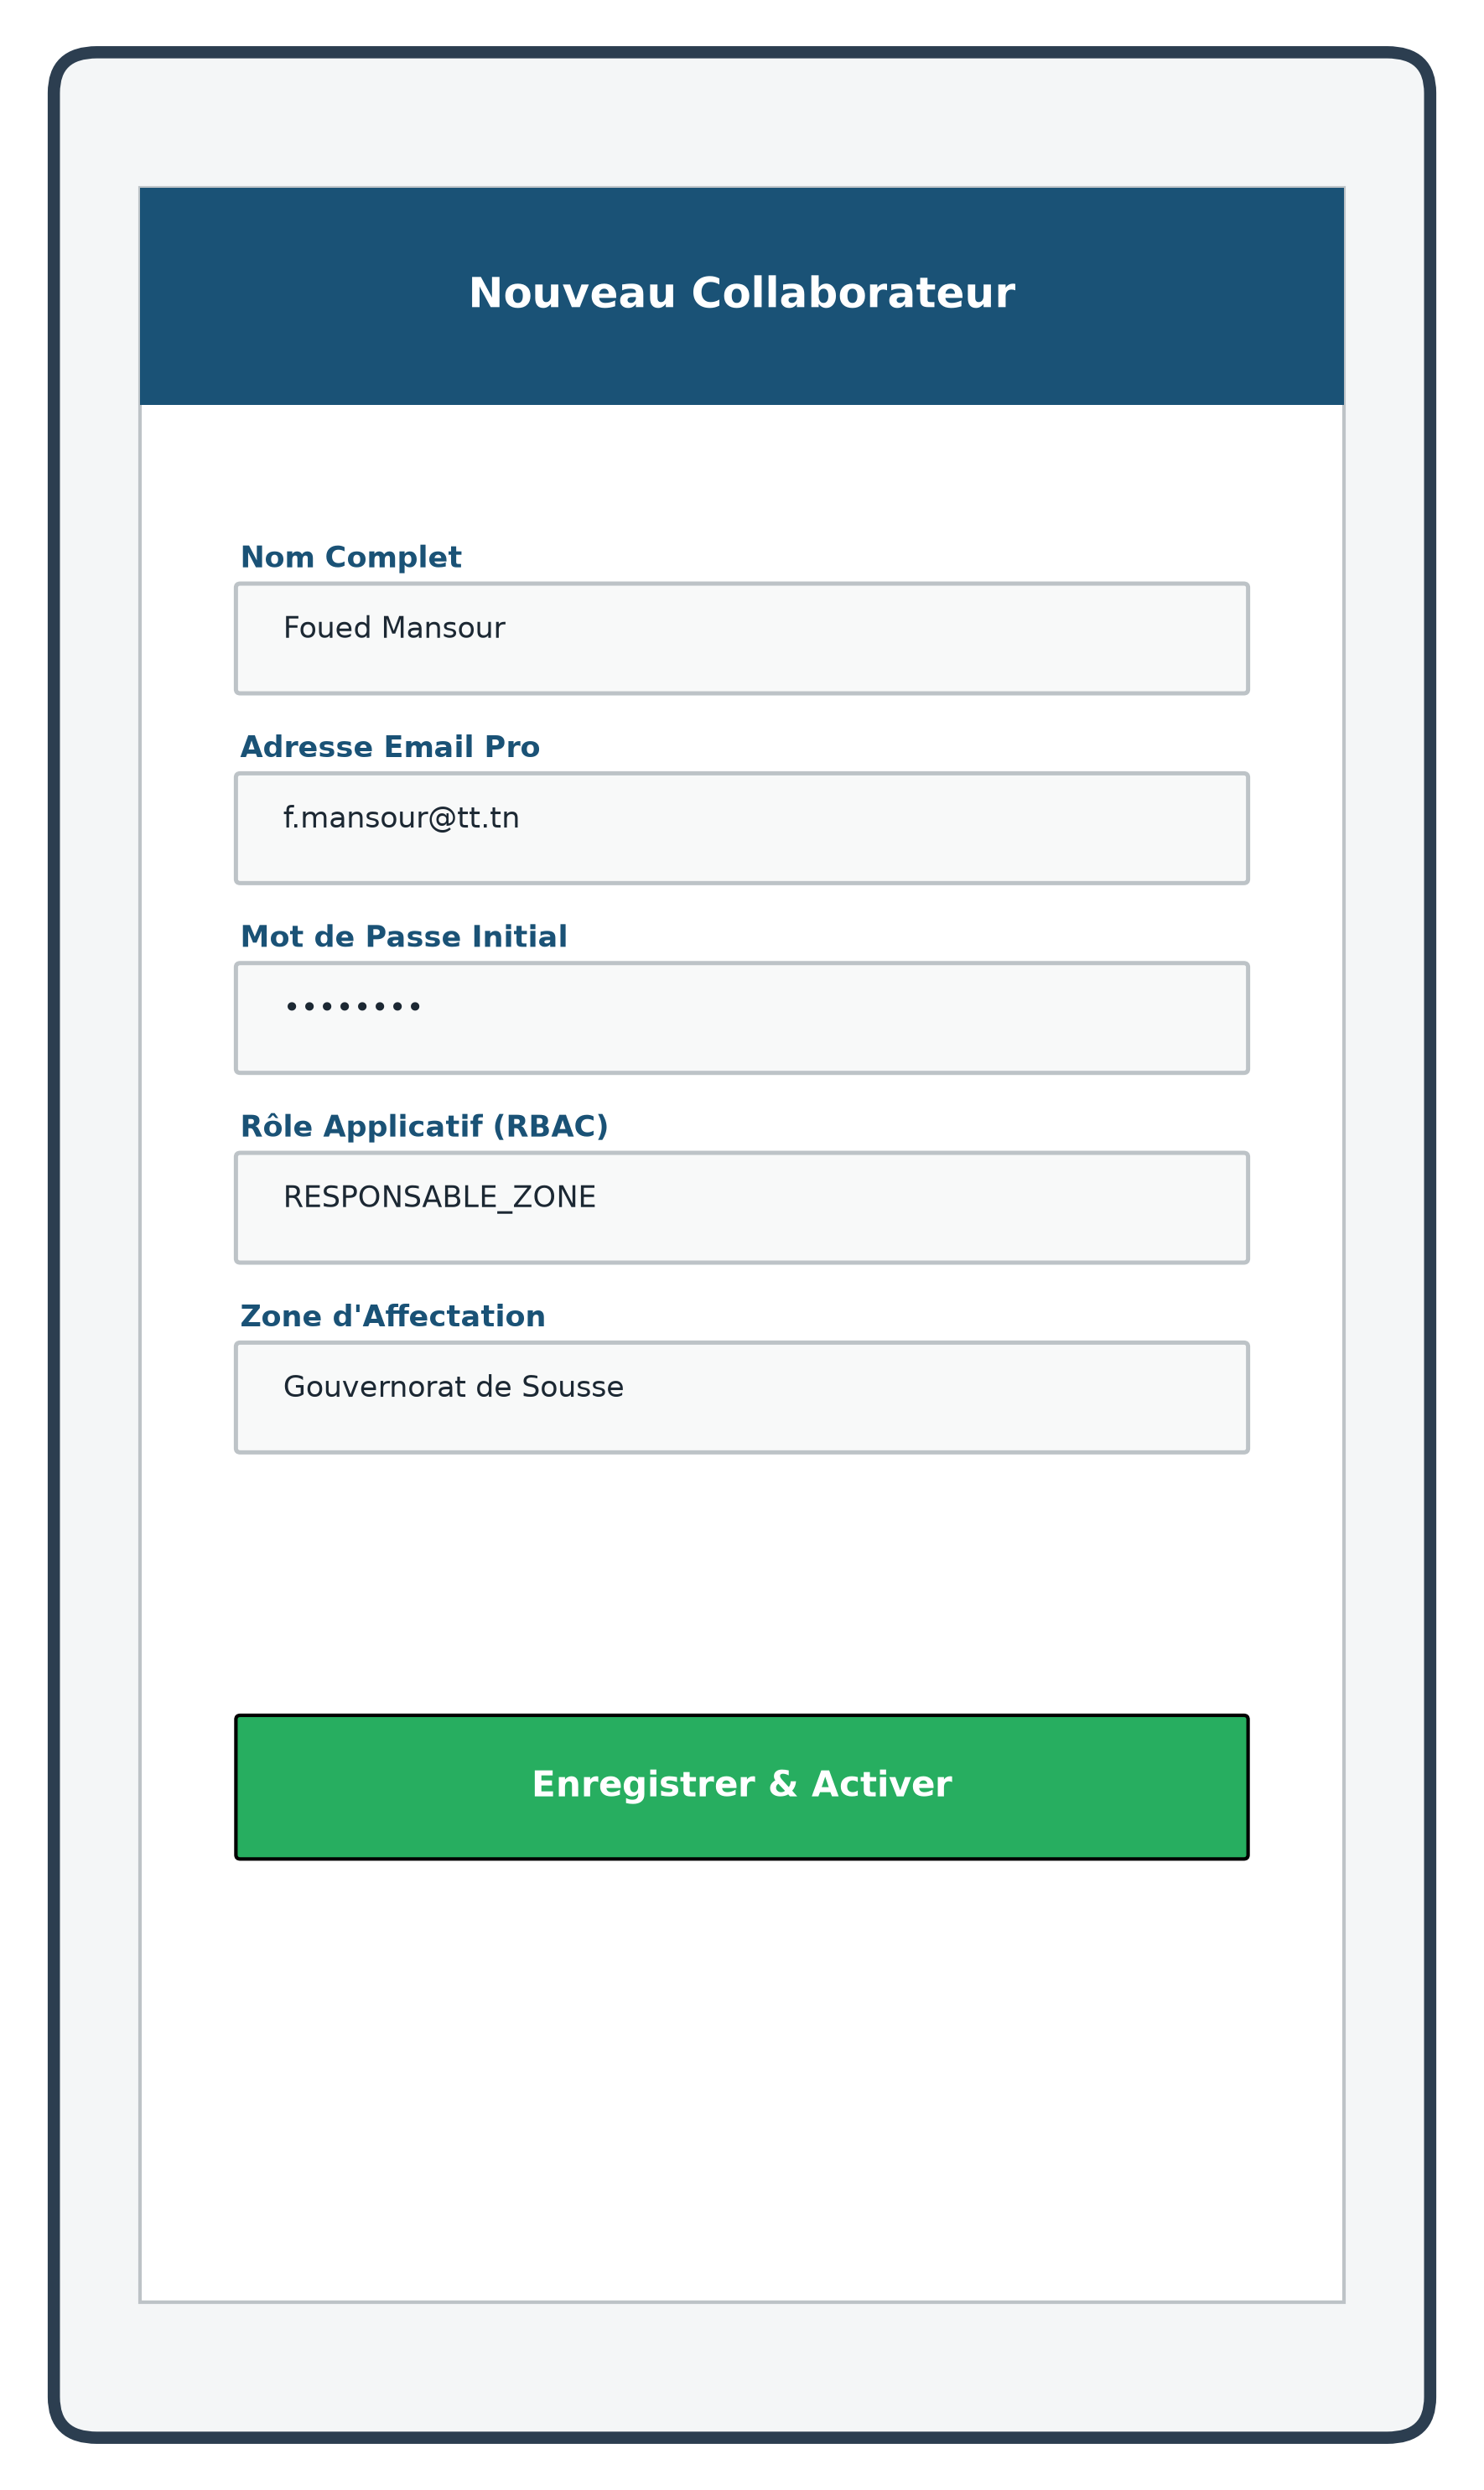
\includegraphics[width=10cm]{Images/ch3/ui_create_user.png}
 \caption{Formulaire de cr\'eation et affectation d'un utilisateur}
 \label{fig:ch3-ui-create-user}
\end{figure}

\section*{Conclusion}
La Release 1 a permis d'\'etablir le socle technique indispensable de la plateforme. La mise en \oe uvre d'une architecture s\'ecuris\'ee JWT/RBAC et d'un syst\`eme d'administration fluide des comptes utilisateurs garantit la fiabilit\'e et la confidentialit\'e des acc\`es. Ce socle pr\'epare le d\'eveloppement des fonctionnalit\'es m\'etier c\oe urs pr\'esent\'ees dans le chapitre suivant : la supervision cartographique et le traitement d'\'ev\'enements en temps r\'eel.
